\chapter{Implementation} \label{chap:implementation}

\section*{}

This chapter presents the implementation of the framework. It starts by 
describing the methodology followed in the realization of the dissertation. It 
is followed by the identification of requirements, the architecture of the 
framework, a study on the scalability of the solution and it is finalized by 
the description of the technology used in the implementation.

\section{Methodology} \label{sec:meth}

Like any software development project, a simulation project also has a life 
cycle. In this section we describe the steps to apply in the simulation 
methodology, based on Ulgen et al.~\cite{Ulgen1994} and Banks et 
al.~\cite[section 1.11]{Banks2004}, which can be summarized as follows:

\begin{enumerate}
    \item \textit{Problem formulation}: Clear statement of the problem by the 
    analyst and stakeholders; \label{enum:mform}
    \item \textit{Setting of objectives and overall project plan}: Questions to 
    be answered by the simulation, plans for the study, cost and number of days 
    for each phase, with the results expected at each stage; \label{enum:mobj}
    \item \textit{Model conceptualization}: Select, modify and iterate over the 
    assumptions that characterize the system; \label{enum:mconcept}
    \item \textit{Data collection}: Collect the necessary data to run and 
    validate the model, assuming that required data will change with the 
    increasing complexity of the system; \label{enum:mdata}
    \item \textit{Model translation}: Materialization of the system in a 
    program; \label{enum:mtransl}
    \item \textit{Verification}: Making sure that the program behaves correctly 
    accordingly to its inputs; \label{enum:mverif}
    \item \textit{Validation}: Calibration of the model, comparing the model 
    against an actual system; \label{enum:mvalid}
    \item \textit{Experimental design}: Tweak the experiments, comparing 
    alternative designs; \label{enum:mexp}
    \item \textit{Production runs and analysis}: Estimate measures of 
    performance for the systems that are being simulated; \label{enum:mprod}
    \item \textit{Documentation and reporting}: Document both the program and 
    the progress of the study; \label{enum:mdocs}
    \item \textit{Implementation}: End result of the study, including the 
    entire simulation process. \label{enum:mimpl}
\end{enumerate}

This process can be visualized in figure \ref{fig:sim}.

\begin{figure}[p]
    \begin{center}
        \leavevmode
        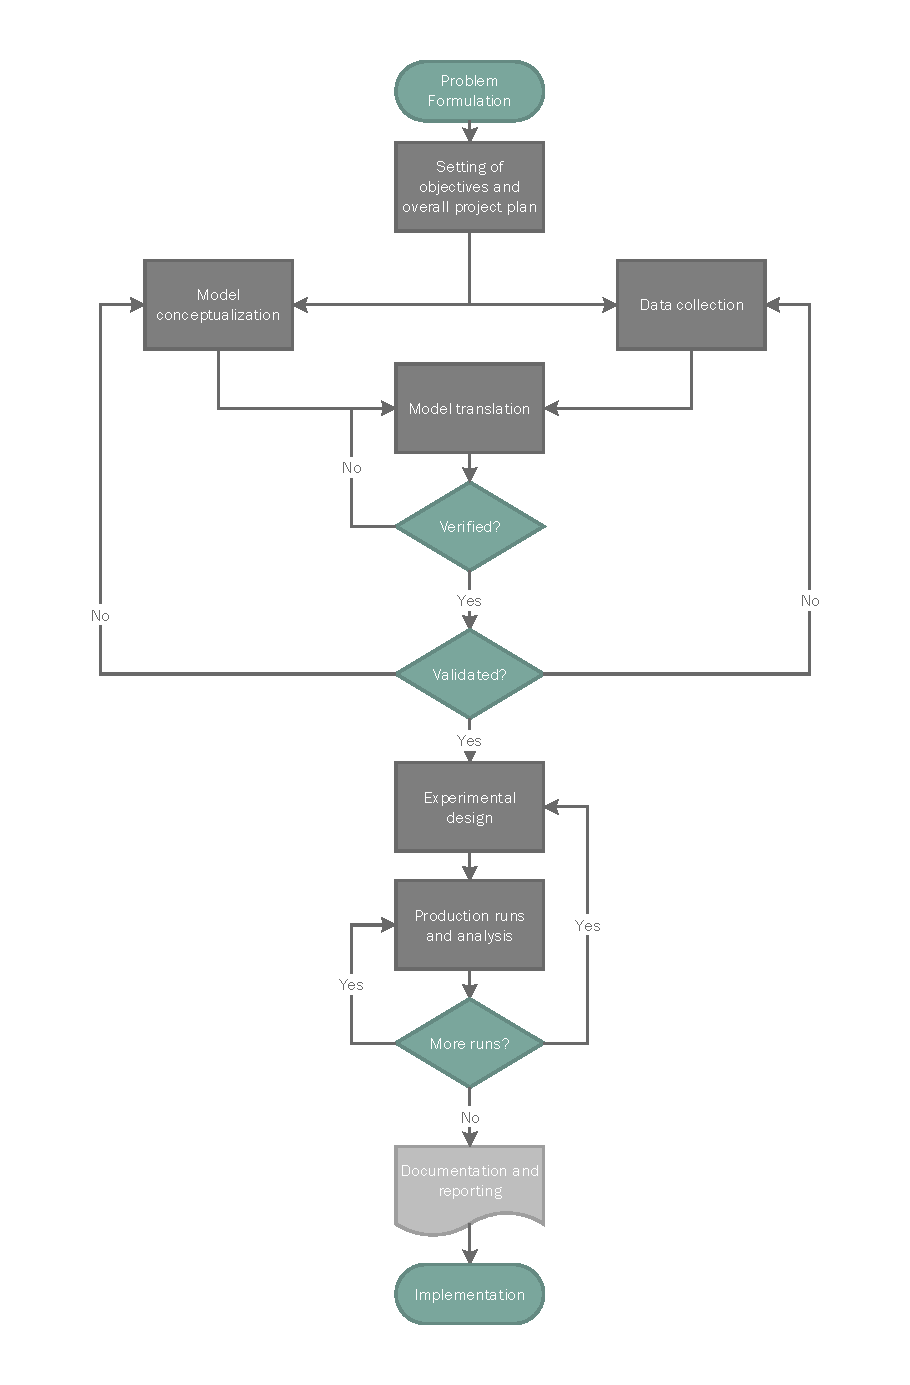
\includegraphics[width=0.95\textwidth]{simulation_study}
        \caption{Steps in a simulation study \cite{Banks2004}}
        \label{fig:sim}
    \end{center}
\end{figure}

\todo{why?}

\section{Requirements}

We have looked at several e-commerce websites, both national and 
worldwide, like Amazon\footnote{\url{https://www.amazon.com/}}, 
eBay\footnote{\url{http://www.ebay.com/}}, 
PCDIGA\footnote{\url{https://www.pcdiga.com}}, 
Clickfiel\footnote{\url{http://clickfiel.pt/}}, 
KuantoKusta\footnote{\url{http://www.kuantokusta.pt/}}, and analysed features 
and characteristics common to all of them, in order to better assess what the 
framework should be able to represent and model. To keep things simple and 
realistically implementable in the given time frame, some limitations had to be 
done. This section lists the requirements and assumptions of the framework.

\subsection{Website Representation}

\begin{itemize}
    \item A website is a collection of web pages;
    \item The common entry point is named homepage but it is possible to enter 
    the website directly from a different page;
    \item Structure and navigation between pages is done with links;
    \item Pages have a purpose like displaying information about a 
    product, listing multiple products, informing about warranty and payment of 
    products and services, etc.. We categorize the pages by using tags;
    \item Product pages have, at least, the product name, its description and 
    price;
    \item A virtual shopping cart is used as a staging area for the products 
    that are going to be bought;
    \item Checkout is the act of taking all the products in the shopping cart 
    and effectively buying and paying them;
    \item Usually, a customer has to create an account and login in the website 
    in order to buy something or access restricted pages.
\end{itemize}

\subsection{Navigation Agents}

\begin{itemize}
    \item Navigation agents represent users or costumers interacting with a 
    website;
    \item Some common interactions are:
    \begin{itemize}
        \item jumping from page to page (or browsing);
        \item exiting the website;
        \item adding a product to the shopping cart;
        \item checking out;
        \item rating a product;
        \item writing a review or comment;
        \item bidding on a product;
        \item filling out forms (login, addresses, bank information, etc.);
        \item comparing two products side by side.
    \end{itemize}
\end{itemize}

\subsection{Website Agents}

\begin{itemize}
    \item Website agents can modify any page before it is \textit{served} to a 
    user/customer;
    \item Example use cases:
    \begin{itemize}
        \item Recommend products to the user based on its preferences or 
        browsing behaviour;
        \item Targeted flash sales or promotions;
        \item A/B testing analysis.
    \end{itemize}
\end{itemize}

\subsection{Simulation Engine}

\begin{itemize}
    \item Given a website, the type of navigation and website agents and 
    pretended simulation time, the simulation can be started, stopped and store 
    its state and calculated metrics in a database.
    \item A simulation run can have thousands of navigation agents entering the 
    simulation at each step;
    \item A simulation run can have one or more website agents.
\end{itemize}

\subsection{Reporting}

\begin{itemize}
    \item Once a simulation run ends, it can be analysed by taking a look at 
    its results, metrics and other previously stored characteristics;
    \item At least two simulation runs can be put side and by side so they can 
    be quickly compared;
    \item The calculated metrics should be relevant to the business, some 
    examples are \cite{Watson2015}:
    \begin{itemize}
        \item Bounce rate
        \item Conversion rate
        \item Total/average order value
        \item Average order value
        \item Items per order
        \item New visitor conversion rate
        \item Shopping cart sessions
        \item Shopping cart conversion rate
        \item Shopping cart abandonment rate
        \item Average session length
        \item Number of browsing sessions
        \item Page views per session
        \item Product views per session
    \end{itemize}
\end{itemize}

\subsection{Limitations}

Some requirements did not make it to the actual implementation:

\begin{itemize}
    \item Adding a product to the cart and the checkout are a single step;
    \item There are no customer accounts, logins, registration, sign ups or 
    sign ins;
    \item Visual information about the pages and products is not represented, 
    e.g., a customer cannot pick a product to by because its associated 
    picture is \textit{appealing};
    \item It is not possible to remove an item from the cart;
    \item Interactions with the website are limited and "hard coded" (listed 
    in sub-section \ref{ssec:multiagents}), not extensible;
    \item The metrics gathered during the simulation are limited, we have 
    implemented some of the metrics listed above, non exhaustively.
\end{itemize}

\section{Architecture}

\subsection{Multi-agent Architecture}\label{ssec:multiagents}

The simulation framework encompasses two different kinds of agents, navigation 
agents and website agents, as shown in figure \ref{fig:agent_arch}.

\begin{figure}[!h]
    \begin{center}
        \leavevmode
        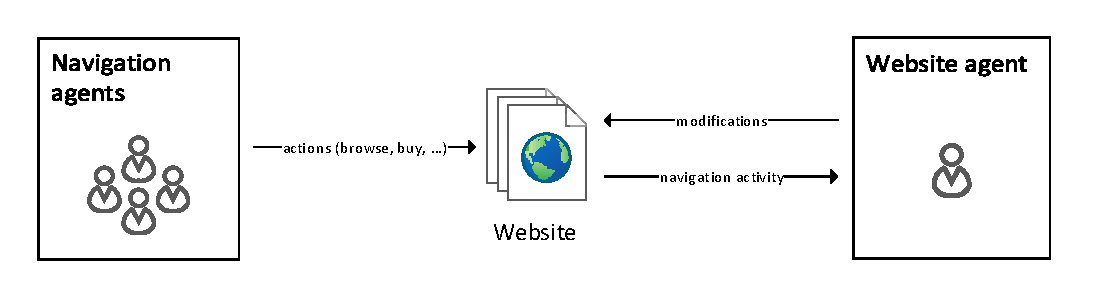
\includegraphics[width=0.95\textwidth]{agent_architecture}
        \caption{Agent interaction with the environment}
        \label{fig:agent_arch}
    \end{center}
\end{figure}

Navigation agents represent users interacting with the website. They have a 
limited view of the system: they have access to the website (pages and links 
between them) and they know the current page they are visiting. Each simulation 
step, the framework asks each navigation agent which action will they pick. The 
action may be to visit another page (\texttt{BrowseToAction}), exit the 
website (\texttt{ExitAction}), add a product to the cart 
(\texttt{AddToCartAction}), finish the purchase (\texttt{CheckoutAction}) 
or simply do nothing (\texttt{IdleAction}). Also related to the navigation 
agents subsystem, an implementation of \texttt{NavigationAgentFactory} is 
used to decide how many navigation agents are added to the system in each step. 
For example, a simplistic implementation might create a fixed number of 
navigation agents or a different one closer to reality could follow a Poisson 
distribution model \cite{gunduz2003poisson}.

Website agents are able to modify the pages before they are served to the 
users. They have a broader view of the system than navigation agents. They are 
notified of all the actions that navigation agents do. The most common use 
case of the website agents is to recommend products to the users: before the 
page is served to a user, a website agent can modify a section of the page to 
display a custom list of products, based on the previous activity of the other 
users or preferences of the current user. However they are not limited to only 
recommendations, a website agent might replace a page's content entirely, 
increase or decrease the price of products (e.g promotions, sales), do nothing, 
etc.

The framework does not assume how these agents behave however the interactions 
between them are limited. The agents do not send messages between each other 
and may only interact indirectly, through the framework (e.g a website agent 
modifies a page before it is "seen" by a navigation agent). While a simulation 
run might have hundreds or thousands of navigation agents, to simplify, each 
run only has one website agent instance (this does not impose a limit on the 
solution, the agent can still be modelled after a composite agent\footnote{An 
    agent that represents multiple composite or virtual agents (our name)}).

It is out of the scope of the framework to provide concrete implementations of 
the agents but we provide 2 implementations of navigation agents and 3 
implementations of website agents, as a way to validate and verify the 
simulation runs. This will be further discussed in 
chapter~\ref{chap:validation}.

\subsection{Simulation Engine}

The simulation engine follows a fairly standard and simple discrete event 
simulation architecture, as described in \ref{ssec:des}. The domain model we 
are dealing with allows certain simplifications of the simulation:

\begin{itemize}
    \item the event list only contains events scheduled for the next step;
    \item there are no conditional events (type C \cite{pidd1998computer});
    \item all the events happen instantaneously;
    \item the events do not depend on other events, they do not require 
    synchronization and may be implemented in a single-threaded engine.
\end{itemize}

The process that the simulation engine follows is described next. In each 
simulation 
loop, the engine starts by calling \textproc{newNavigationAgents()} which adds 
new navigation agents to the simulation. The number and type of these agents 
are decided by the \texttt{NavigationAgentFactory}. After that, each 
navigation agent currently active (i.e did not leave the website) chooses an 
action to do (buy, browse, etc.). Depending on the action that 
was picked, the engine updates its internal state. The simulation state is 
represented by \texttt{WebsiteState} and contains statistics and other 
performance metrics. Whenever the picked action implies presenting the 
navigation agent a page from the website, the website agent can modify that 
page before it is presented, by calling \textproc{modifyPage(navAgent, page)}. 
The website agent is also notified about all actions that the navigation agents 
do (\textproc{notify(navAgent, action)}). The simulation is configured to end 
after a fixed number of steps, otherwise it could run forever.

This process is illustrated in figure \ref{fig:sequence_diagram}. 

\begin{figure}[h]
    \begin{center}
        \leavevmode
        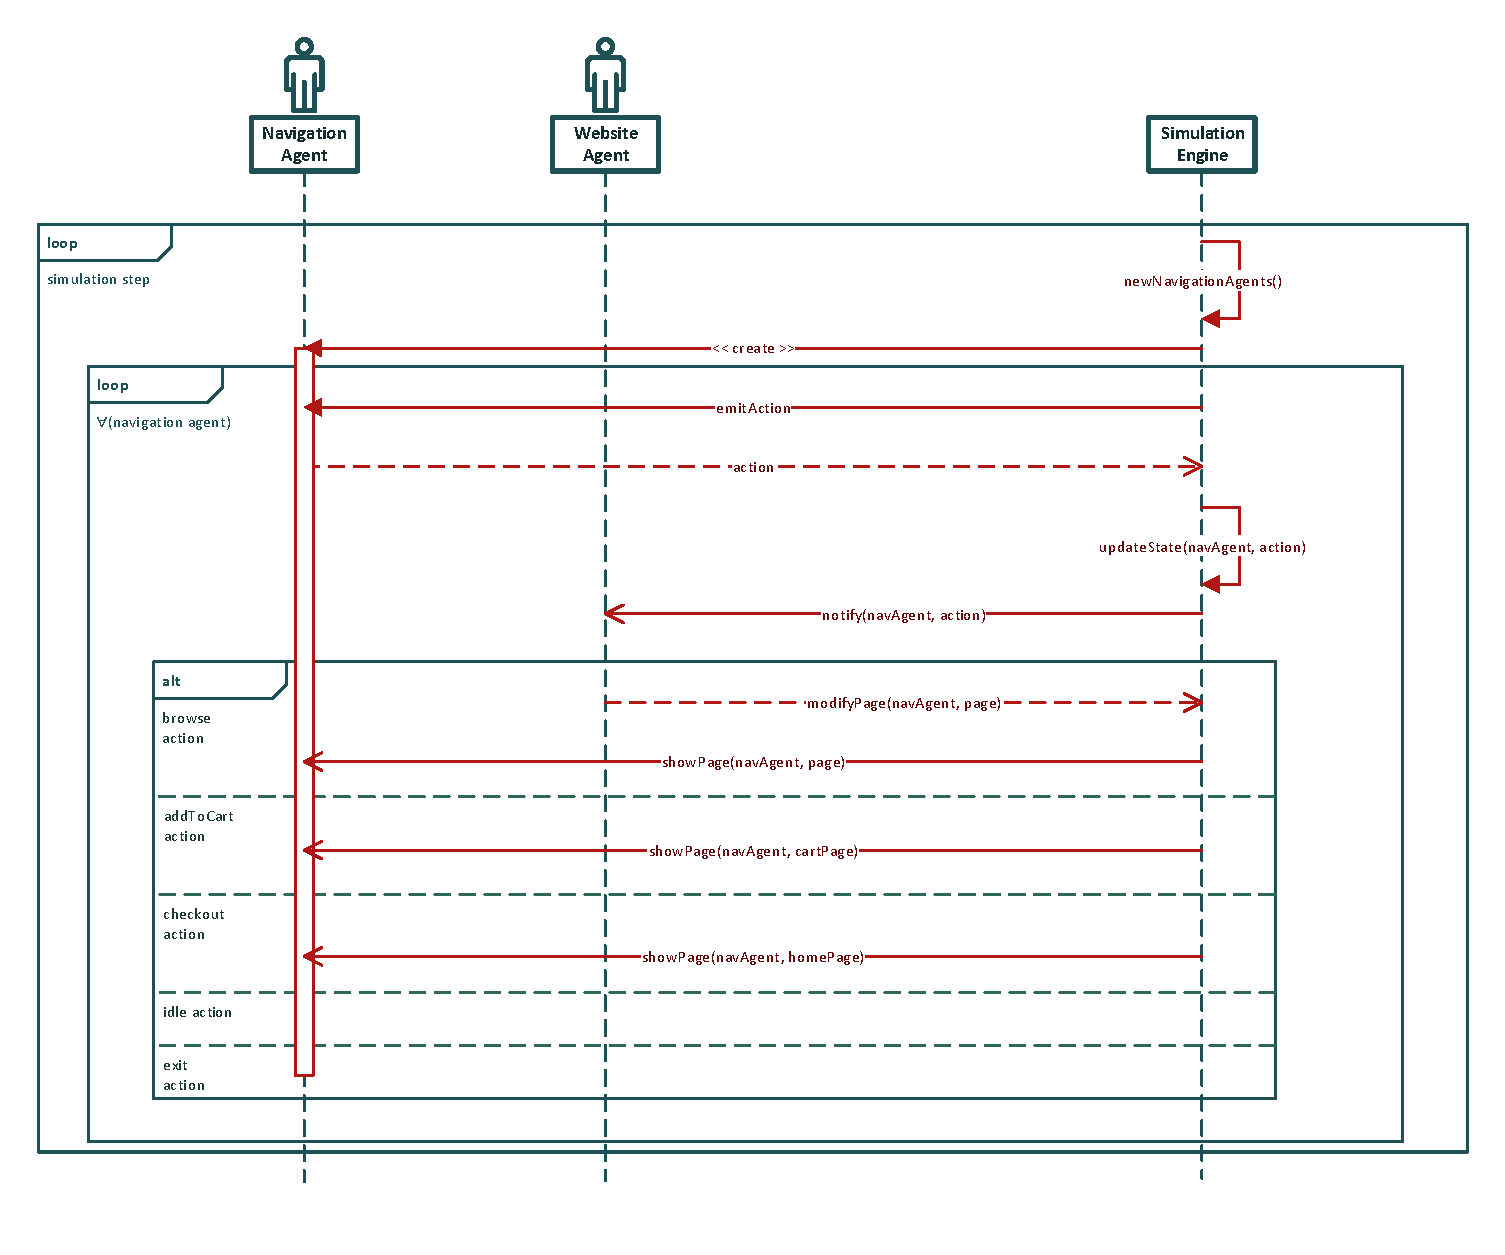
\includegraphics[width=0.95\textwidth]{sequence_diagram}
        \caption{Sequence diagram for the simulation engine}
        \label{fig:sequence_diagram}
    \end{center}
\end{figure}

\subsection{Class Model}

In this sub-section we describe all the classes used to represent all the 
entities in the simulation engine (figure \ref{fig:class}).

\texttt{Website} represents a website, it contains a set of \texttt{pages} and 
a reference to its \texttt{homepage}, the entry point of the website. A 
\texttt{Page} has a set of \texttt{links}, which are all the outbound 
hyperlinks that a page contains, it has a set of \texttt{tags}, which is used 
to categorize a page (e.g electronics category, clothing category, cart page, 
product search page, etc.) and the page may also contain a \texttt{Product}, if 
the page is a product page. A \texttt{Product} has a \texttt{name}, a 
\texttt{description} and a \texttt{price}.

The \texttt{Simulation} is an abstract class that contains an \texttt{agenda} 
which stores all the \texttt{Action}s (an arbitrary function) to be executed in 
the next steps. It provides a way to enqueue work in the simulation using 
\textproc{schedule(delay, action)} and a \textproc{run()} method that consumes 
the \texttt{agenda} until there's no more work to do. A subclass of 
\texttt{Simulation}, \texttt{WebsiteSimulation} represents a simulation 
happening over websites. It contains the \texttt{Website} itself, a 
\texttt{WebsiteState}, a \texttt{NavigationUserFactory} and a 
\texttt{WebsiteAgent}. The \texttt{WebsiteState} is used to keep track of all 
the statistics and metrics that the simulation produces. This state can be 
stored in a database to analyse the results once the simulation is finished.

\texttt{NavigationAgent} is an interface that represents users interacting with 
the website. Implementations of it have to implement \textproc{emitAction}, 
which returns the \texttt{Action} the agents wants to do based on their 
internal state and their current page. These agents are added to the simulation 
by an implementation of \texttt{NavigationAgentFactory}. \texttt{WebsiteAgent} 
is an interface that represents the agents that may modify the website and that 
are notified about all the navigation agent activity. The code for these three 
interfaces is displayed in listing \ref{src:agentsinterfaces}.

The mutability of the system is contained to the \texttt{Simulation} (due to 
its \texttt{agenda}) and \texttt{WebsiteState} which is updated every 
simulation step.

The points of extensibility of the framework are the agents interfaces 
(\texttt{NavigationAgent}, \texttt{NavigationAgentFactory} and 
\texttt{WebsiteAgent}) and \texttt{WebsiteState} (e.g provide additional 
tracking metrics or visualizations).

\begin{figure}[p]
    \begin{center}
        \leavevmode
        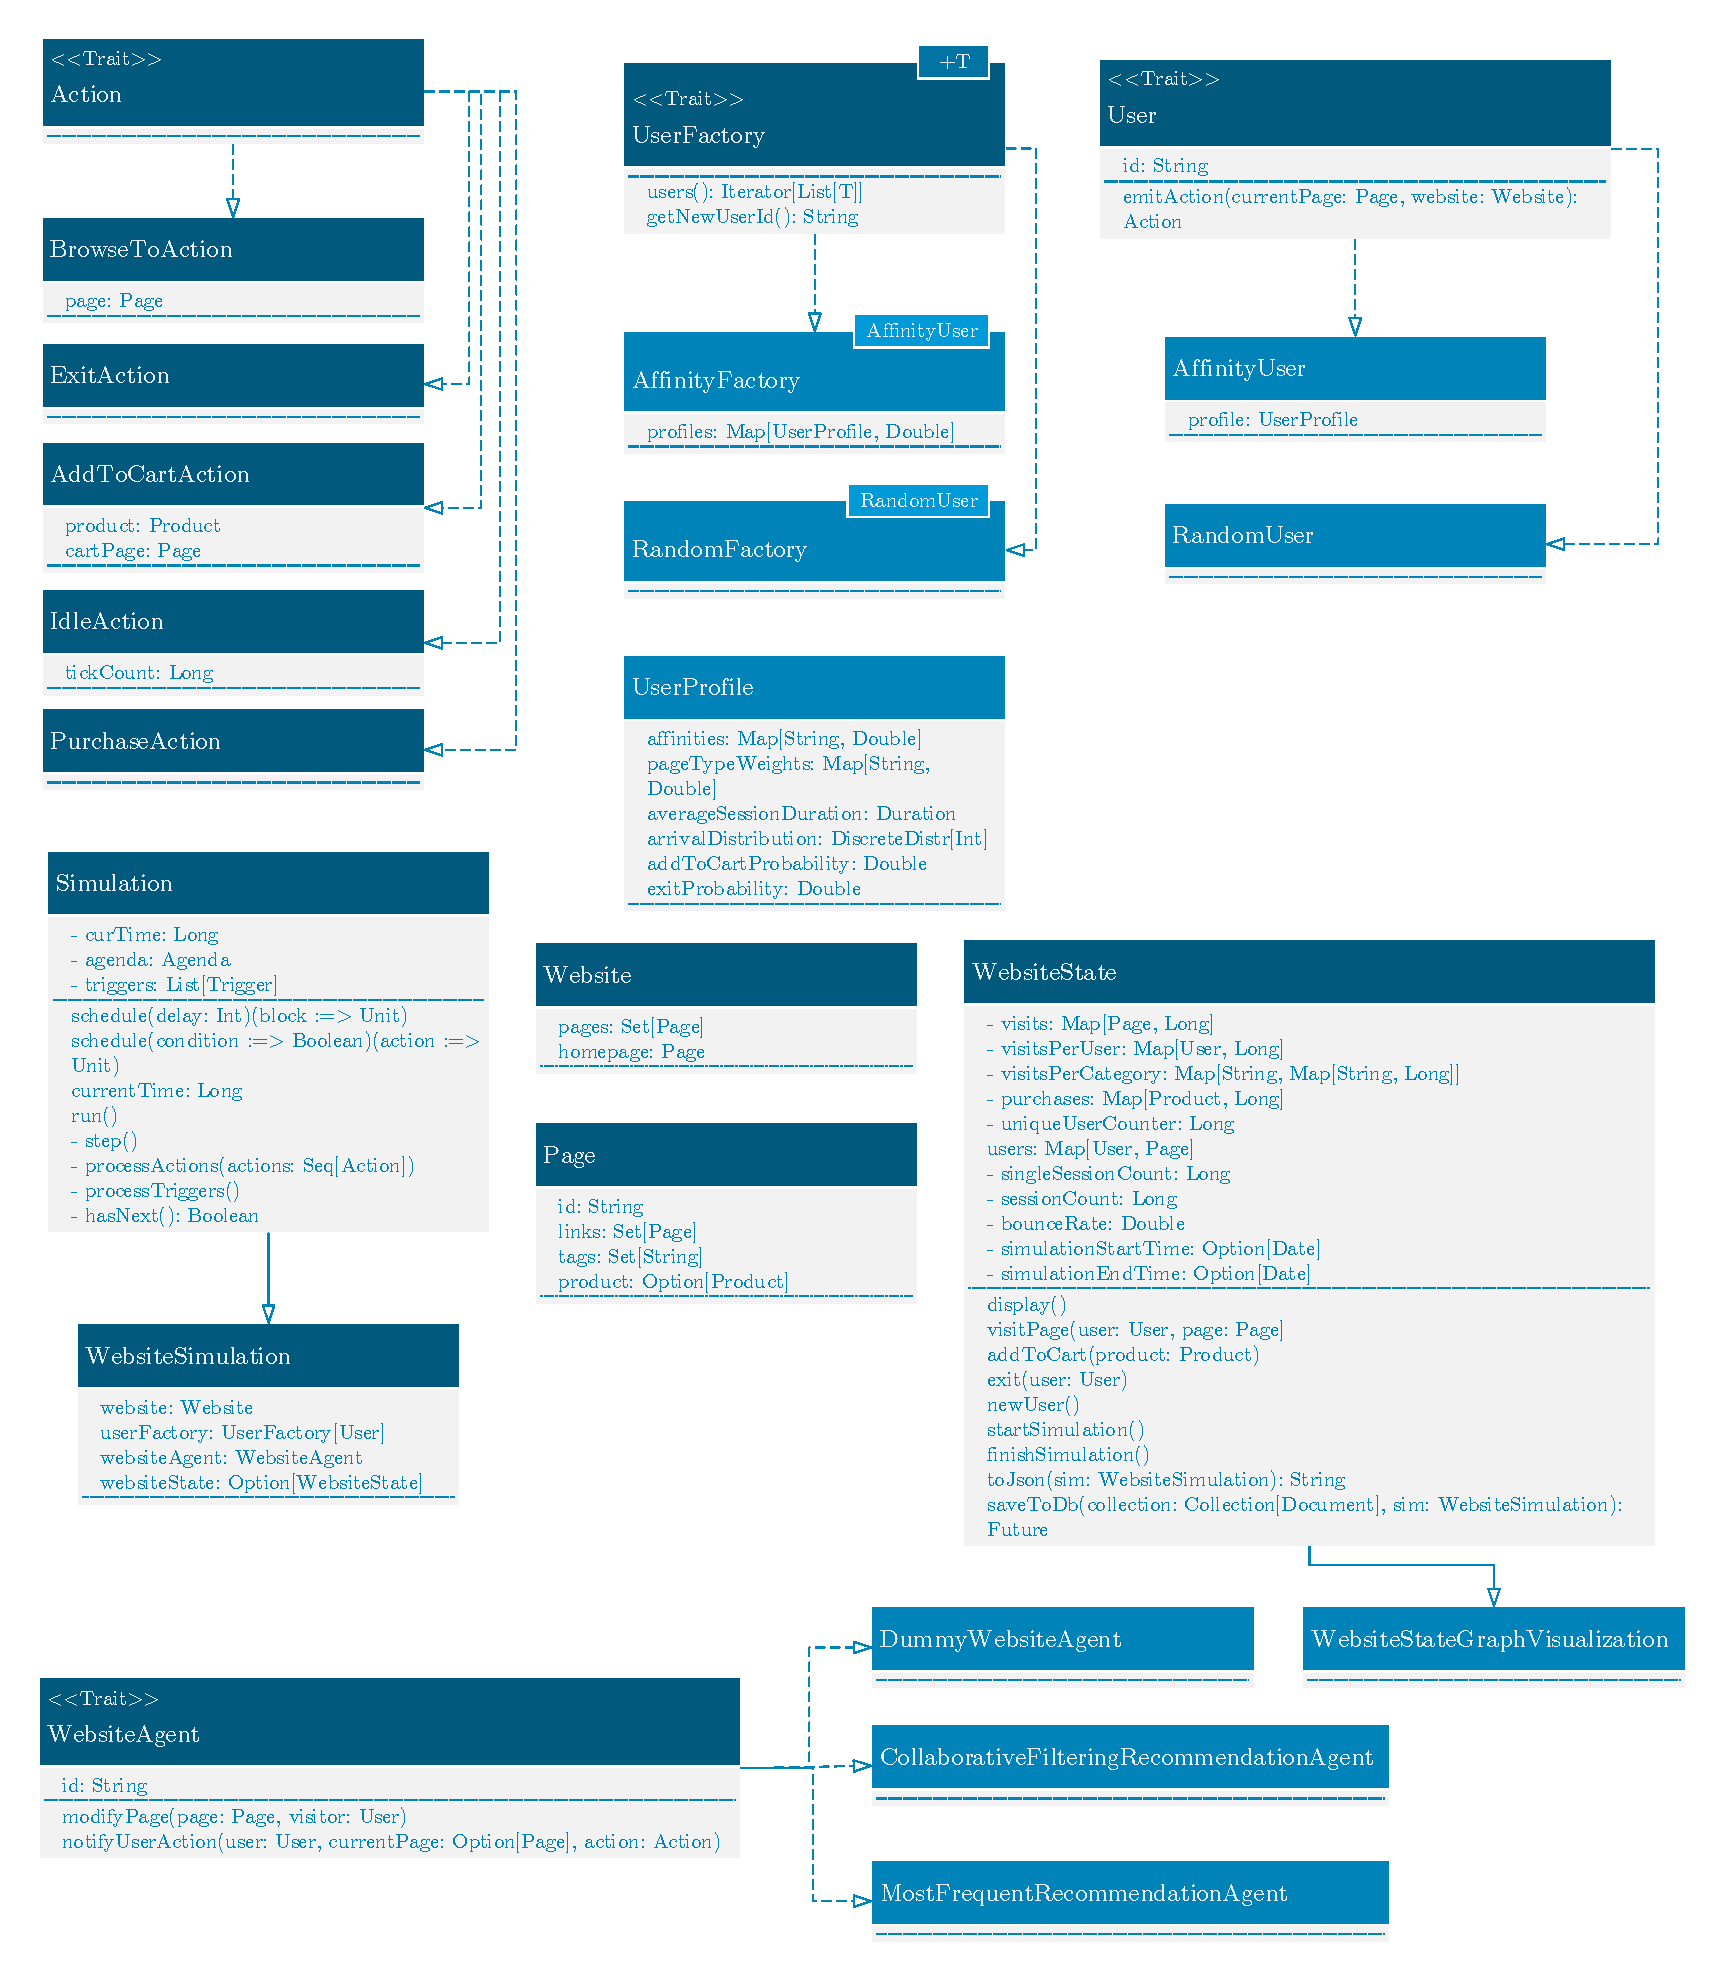
\includegraphics[width=1\textwidth]{class_diagram}
        \caption{Class diagram}
        \label{fig:class}
    \end{center}
\end{figure}

\todo{fix class diag}

\begin{lstlisting}[float,language=Scala, label=src:agentsinterfaces, 
caption=Definition of the agents interfaces]
trait NavigationAgentFactory[+T] {
    def users: Iterator[List[T]]
}

trait NavigationAgent {
    def emitAction(currentPage: Page, website: Website): Action
}

trait WebsiteAgent {
    def modifyPage(page: Page, user: NavigationAgent): Page
    def notifyUserAction(user: NavigationAgent, currentPage: Option[Page], 
                         action: Action)
}

\end{lstlisting}

\subsection{Graphical User Interface}

A frontend website has been developed to aid in displaying and visualizing the 
results of each simulation run. The data is loaded asynchronously from a 
database which stores \texttt{WebsiteState} snapshots. All the data is rendered 
to the user server-site except the data required to display charts (e.g Visits 
per Category chart).

The interface has three distinct views: a simulation list, details about a 
simulation run and comparison between two simulation runs:

\begin{itemize}
    \item The simulation list view (\texttt{\textbf{GET} /simulations}) (figure 
    \ref{fig:sim_view}) displays a table 
    with all the simulation runs stored in the database. It shows the 
    identifier, name, agent types and timestamp of each run.
    \item The detail view (\texttt{\textbf{GET} /simulations/\textit{<id>}}) 
    (figure \ref{fig:sim_detail_view})
    display information regarding a single simulation run. This info describes 
    the simulation and it contains data regarding the types of the agents used, 
    start and finish time of the simulation, collected metrics (e.g bounce 
    rate, conversion rate, total order value, etc.), visits per page, visits 
    per page category, purchases per product and others. This information is 
    displayed using mostly tables and charts.
    \item The last view, the comparison page (\texttt{\textbf{GET} 
    /simulations/compare/\textit{<idA>}/\textit{<idB>}}) (figure 
    \ref{fig:sim_compare_view}) displays information 
    regarding two simulation runs (A and B) side by side, so they can be 
    compared and analysed. The planned use case of this view is to quickly spot 
    differences between two runs and see how different agent configurations 
    affect the results.
\end{itemize}


\section{Scalability}\label{sec:scalability}

To assess the scalability and performance of the simulation engine, some 
benchmarks were made and they are described next. The tests were ran in a 
Windows 10 laptop with a Intel\textregistered~Core\texttrademark~i7-4710HQ CPU 
@ 2.50GHz (8 CPUs) processor. A modified\footnote{Changed each measurement to 
run the same block of code 10 times, drop the first 2 runs and take the average 
of the 8 runs instead of running it only once.} version of the library 
Benchmark.scala\footnote{\url{https://github.com/balagez/Benchmark.scala}} was 
used, which is based on Ruby's Benchmark 
module\footnote{\url{http://ruby-doc.org/stdlib-1.9.2/libdoc/benchmark/rdoc/Benchmark.html}}.
 The focus is not necessarily in the raw speed of the engine but rather in the 
variation of the simulation time when the number of agents in the system or the 
number of steps of the simulation are increased.

The test performed consists of running the same simulation with an 
increasing number of navigation agents and number of simulation steps, set up 
in the following way:

\begin{itemize}
    \item \textbf{Website}: Toy sample website with 9 pages and 32 total links 
    between pages (1 homepage, 1 cart page, 3 product list pages and 4 product 
    pages);
    \item \textbf{Website agent}: Dummy agent, does not modify any page;
    \item \textbf{Navigation agent}: Sample agent implementation which 
    picks the next action randomly. Configured with a chance of exiting the 
    website of $\frac{1}{3}$ and a change of adding a product to the cart of 
    $\frac{1}{20}$;
    \item \textbf{Number of navigation agents}: From 1000 to 10000 with 
    increments of 1000;
    \item \textbf{Number of simulation steps}: From 100 to 1000 with increments 
    of 100.
\end{itemize}

The result of the 100 simulation runs is shown in figure \ref{fig:simbench} 
(whose data is in table \ref{tab:simbench}). A quick analysis shows that the 
simulation time scales linearly ($\bar{R^{2}} = 0.99149, \sigma = 0.00648$) 
with both the number of agents and the number of simulation steps. For 
instance, a simulation with 1000 steps and 10000 navigation agents (entering 
the system each step)	 took 41.95 seconds. These initial results are very 
satisfactory however they should be improved, especially when the number of 
steps is increased, so that simulations that span a longer period of time can 
be evaluated (e.g simulate the effect of seasonal customers over an entire 
year).

\begin{figure}[h]
    \begin{center}
        \leavevmode
        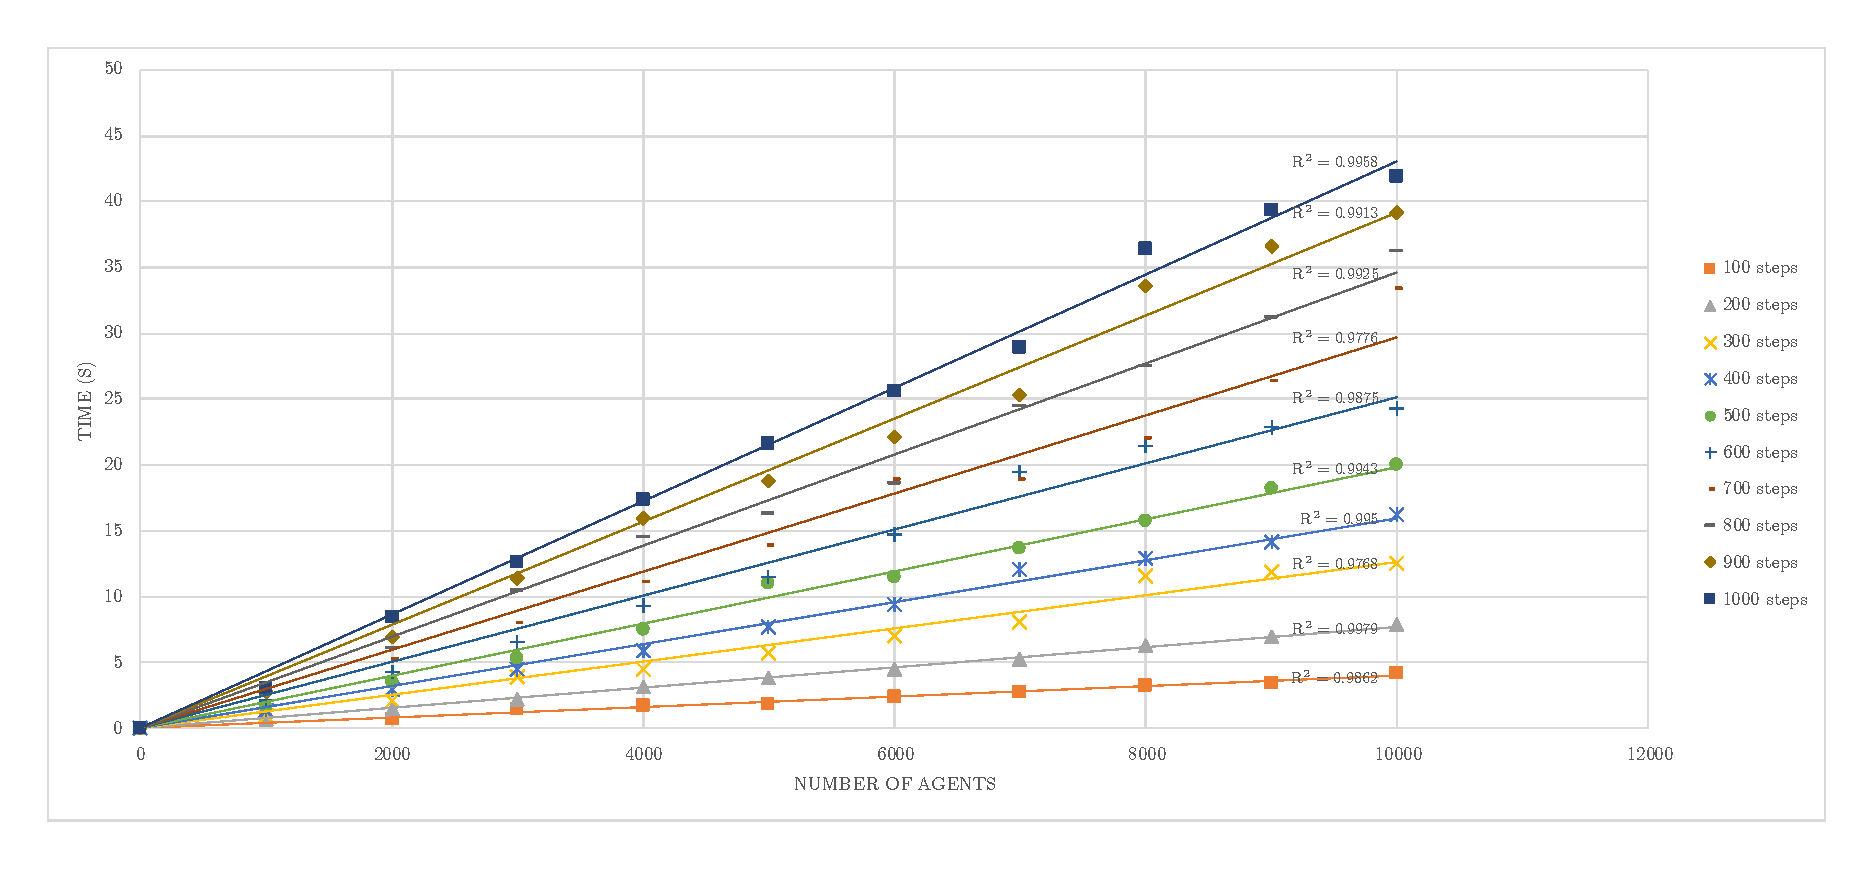
\includegraphics[width=0.95\textwidth]{simulation_benchmark}
        \caption{Simulation running time for different number of 
        navigation agents and simulation steps}
        \label{fig:simbench}
    \end{center}
\end{figure}

\begin{table}[h]
    \centering
    \caption{Simulation running time (in seconds) for different number of 
    navigation agents and simulation steps}
    \label{tab:simbench}
    \begin{tabular}{@{}lllllllllll@{}}
        \toprule
        \diaghead(5, -3){Stepagent}{Steps}{Agents} & 1000 & 2000 & 3000 & 4000 
        & 5000 
        & 
        6000 & 7000 & 8000 & 
        9000 & 10000 \\ \midrule
        100 & 0.62 & 0.69 & 1.45 & 1.72 & 1.81 & 2.34 & 2.76 & 3.23 & 3.42 & 
        4.16 \\
        200 & 0.67 & 1.43 & 2.20 & 3.17 & 3.84 & 4.49 & 5.22 & 6.30 & 6.93 & 
        7.89 \\
        300 & 0.95 & 2.07 & 3.90 & 4.44 & 5.72 & 7.01 & 8.05 & 11.62 & 11.89 & 
        12.53 \\
        400 & 1.32 & 2.91 & 4.42 & 5.88 & 7.69 & 9.39 & 12.01 & 12.93 & 14.15 & 
        16.18 \\
        500 & 1.58 & 3.48 & 5.34 & 7.49 & 11.03 & 11.44 & 13.65 & 15.77 & 18.20 
        & 20.00 \\
        600 & 2.10 & 4.31 & 6.59 & 9.26 & 11.52 & 14.71 & 19.44 & 21.47 & 22.83 
        & 24.29 \\
        700 & 2.55 & 5.24 & 7.97 & 11.14 & 13.89 & 18.91 & 18.89 & 22.04 & 
        26.33 & 33.35 \\
        800 & 2.56 & 6.10 & 10.46 & 14.48 & 16.31 & 18.56 & 24.49 & 27.52 & 
        31.19 & 36.26 \\
        900 & 2.77 & 6.94 & 11.37 & 15.97 & 18.77 & 22.11 & 25.36 & 33.56 & 
        36.57 & 39.21 \\
        1000 & 3.07 & 8.47 & 12.64 & 17.40 & 21.59 & 25.62 & 28.94 & 36.46 & 
        39.40 & 41.95 \\ \bottomrule
    \end{tabular}
\end{table}

% \todo{More tests?}

\section{Technology}

Scala\footnote{\url{http://www.scala-lang.org/}} was the language of choice to 
implement the framework and accompanying projects. Scala is a statically typed, 
general purpose programming language that leverages both object oriented and 
functional programming paradigms, while being fully interoperable with the JVM 
(and Java).

The version of Scala used was 2.11.8 with sbt 
0.13.11\footnote{\url{http://www.scala-sbt.org/}}, the \textit{de facto} build 
tool for Scala projects.

The library Breeze (version 
0.12)\footnote{\url{https://github.com/scalanlp/breeze}} of the 
ScalaNPL\footnote{\url{http://www.scalanlp.org/}} package was used 
for numerical processing and statistics.

Apache Spark\texttrademark1.5\footnote{\url{http://spark.apache.org/}} was used 
to train recommendation models in one of the implementations of website agents. 

GraphStream 1.3\footnote{\url{http://graphstream-project.org/}} was used to 
visualize websites as a dynamic graph.

To store simulation run results, the database MongoDB 
3.2.3\footnote{\url{https://www.mongodb.com/}} was used due to its practicality 
and rapid development.

The frontend was built with the Play Framework 
2.5\footnote{\url{https://www.playframework.com/}}.
